\chapter{Técnicas no lineales. t-SNE, MDS e ISOMAP}

\section{t-SNE (t-Distributed Stochastic Neighbor Embedding)}

\textbf{t-SNE} (\textit{t-Distributed Stochastic Neighbor Embedding}) permite transformar datos de múltiples dimensiones a representaciones bidimensionales o tridimensionales, facilitando la identificación de estructuras y relaciones intrínsecas que serían difíciles de observar en su espacio original.

La idea central de t-SNE es mapear los puntos de datos de alta dimensionalidad en un espacio de menor dimensionalidad, preservando las relaciones locales entre los puntos. Se mide la similitud entre puntos de datos en el espacio de dimensión alta y se representa dicha similitud en función de sus probabilidades. Una vez se tienen las distancias se construye una distribución de probabilidad similar en el espacio de dimensiones inferiores y se minimiza la diferencia entre las dos distribuciones utilizando la técnica del descenso del gradiente. De esta forma se captura de manera efectiva la estructura local de los datos, lo que hace particularmente útil la visualización de datos complejos y el descubrimiento de patrones.

Cuando se habla de preservar las relaciones entre los puntos, se refiere a mantener las distancias relativas y las similitudes entre puntos de datos vecinos cuando se asignan desde un espacio de alta dimensionalidad a un espacio de menor dimensión.

\subsection{Algoritmo de t-SNE}
\begin{enumerate}
    \item Selección del conjunto de datos.
    \item Preprocesamiento y normalización de los datos.

    \item Cálculo de distancias en la dimensión original: t-SNE utiliza probabilidades. Para cada punto de datos, se traza una distribución gaussiana a su alrededor con una media cero y una desviación estándar que se determina en función de la densidad de los puntos cercanos alrededor de un punto $x_1$. En un análisis de datos, se usa el eje X para representar las distancias entre cada punto del conjunto de datos y un punto de referencia específico. En el eje Y se representa la densidad de probabilidad, que indica qué tan probable es que un punto esté a cierta distancia del punto de referencia, utilizando una función de densidad para calcular una puntuación de similitud. Este proceso se repite para todos los puntos del conjunto de datos, generando una matriz de similitudes entre puntos. La distribución de probabilidades es única para cada punto, y las similitudes no son necesariamente simétricas. Un valor alto de probabilidad entre dos puntos indica que están cerca (son vecinos), y un valor bajo que están lejos.


    \item Distribución de probabilidades t-Student: para reducir la dimensionalidad, se distribuyen puntos aleatoriamente en el eje $X$. Se calcula la puntuación de similitud de cada punto con relación a los demás, obteniendo otra matriz de $n\times n$. 


    \item Con las dos matrices de $n \times m$, donde una representa las puntuaciones de similitud en la dimensión superior y la otra representa las puntuaciones de similitud en una dimensión inferior, se define una función de coste basada en la divergencia de Kullback-Leibler entre las distribuciones de alta y baja dimensión. Se alinean la matriz de dimensión inferior con la de dimensión superior, utilizando técnicas de optimización como el descenso del gradiente, para minimizar la función de coste. Esto implica ajustar la posición de los puntos de forma iterativa hasta que la matriz de similitud en la dimensión inferior se parezca lo máximo posible a la de dimensión superior. Dicho de otra forma, se itera hasta que las posiciones de los puntos en el espacio de baja dimensión converjan a una configuración que minimice la función de coste

    
    \item  Visualización y análisis: se generan visualizaciones de los datos en el espacio de baja dimensión, interpretando los resultados y analizando las agrupaciones formadas.
\end{enumerate}


\subsection{Aplicaciones de t-SNE}
\begin{itemize}
    \item Agrupación y clasificación: agrupar puntos de datos similares en dimensiones inferiores. Se suele utilizar para encontrar patrones en los datos.

    \item Detección de anomalías.

    \item Procesamiento del lenguaje natural: visualiza incrustaciones de palabras generadas a partir de un gran corpus de texto que facilita la identificación de similitudes y relaciones entre palabras.

    \item Seguridad informática: se pueden visualizar patrones de tráfico de red y detectar anomalías.

    \item Investigación del cáncer: para visualizar perfiles moleculares de muestras de tumores e identificar subtipos de cáncer.

    \item Interpretaciones geológicas: visualización de atributos sísmicos e identificación de anomalías geológicas.

    \item Procesamiento de señales biomédicas: para visualizar electroencefalogramas y detectar patrones de actividad cerebral.
\end{itemize}

\subsection{Ventajas y desventajas}
\begin{itemize}
    \item Ventajas: Si se aplica correctamente, puede ofrecer visualizaciones muy intuitivas preservando la estructura local de los datos en las dimensiones inferiores.

    \item Desventajas:  Es costoso computacionalmente. No es muy bueno preservando la estructura global. Sensible a hiperparámetros. Puede quedarse atascado en los mínimos locales. La interpretación puede ser un desafío.
\end{itemize}

\section{t-SNE vs PCA}

Ambas son técnicas de reducción de la dimensionalidad. PCA funciona mejor con datos lineales; busca identificar los componentes principales subyacentes en los datos proyectándolos en dimensiones inferiores, minimizando la variación y preservando grandes distancias por pares. t-SNE se preocupa por preservar pequeñas distancias por pares, mientras que PCA se enfoca en mantener grandes distancias por pares para maximizar la varianza.

\section{Multi-Dimensional Scaling (MDS)}
El \textbf{escalado multidimensional (MDS)} es una herramienta estadística que ayuda a descubrir conexiones entre puntos en un espacio de dimensiones más bajo que las dimensiones originales. Utiliza técnicas de análisis de datos de similitud o disimilitud canónica.

El objetivo principal es mantener las proximidades originales entre conjuntos de datos; los datos más similares se ubican muy cerca unos de otros, mientras que los datos más separados se colocan separados en el espacio de dimensión menor.

Existen tres tipos de escala multidimensional: 
\begin{itemize}
    \item  \textbf{Algoritmo clásico}: toma una matriz de entrada que representa diferencias entre pares de elementos y produce una matriz de coordenadas que minimiza la dimensionalidad.

    \item Escalamiento multidimensional métrico que generaliza el procedimiento de optimización a varias funciones de pérdida y matrices de entrada con distancias y pesos desconocidos. Minimiza una función de coste llamada «stress».

    \item  Escalado multidimensional no métrico: encuentra la relación monótona no paramétrica entre las diferencias y distancias euclidianas entre elementos, junto con la ubicación de cada elemento en el espacio de baja dimensionalidad. Se define una función de «stress» a optimizar y se considera que es monótonamente creciente.
\end{itemize}


\section{Isometric mappping (Isomap)}

Mapeo isométrico o Isomap combina varios algoritmos que le permiten utilizar una forma no lineal para reducir las dimensiones preservando las estructuras locales. 

\subsection{Algoritmo de Isomap)}

\begin{enumerate}
    \item Se utiliza KNN para encontrar los $K$ vecinos más cercanos de cada punto del conjunto de datos.
    \item Se construye un grafo de vecindad conectando solo los puntos que son vecinos; los demás quedan desconectados.
    \item Se calcula la distancia geodésica entre todos los pares de puntos usando algoritmos como Floyd-Warshall o Dijkstra.
    \item Se aplica escalado multidimensional (MDS) para incrustar los puntos en un espacio de menor dimensión, preservando las distancias geodésicas.
\end{enumerate}


\section{Comparativa de todas las técnicas de reducción de dimensionalidad}

\begin{figure}[ht]
    \centering
    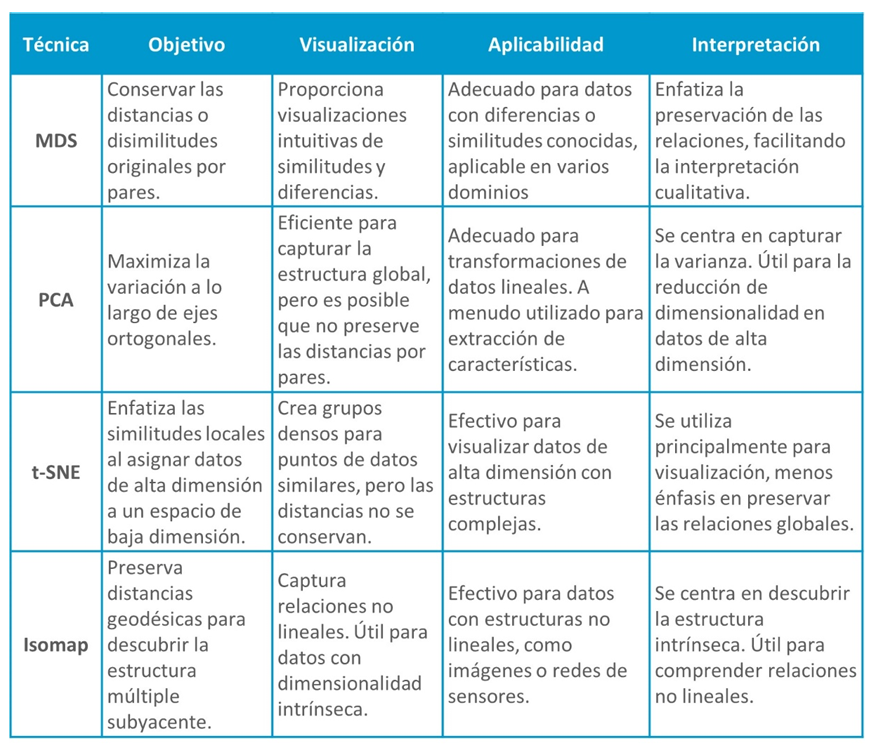
\includegraphics[width=1\linewidth]{imagenes/comparativa-reduccion-dim.png}
    \label{fig:comparativa-reduccion-dim}
\end{figure}